\mnDifficult\begin{slikaDesno}{fig/klatno_1.pdf}[fig/klatno_2.pdf]
    \PID 
    У механичком систему са слике \ID.1 приказано jе инверзно клатно причвршћено
    за ослонац коjи може да се креће дуж $x$ осе. Клатно jе сачињено из кугле масе
    $m$, чиjи jе центар на растоjању $L$ од ослонца, а слободно jе да се креће у равни
    цртежа. Познато jе и $g = |{\bf g}|$.
    \begin{enumerate}[label=(\alph*)]
        \item Одредити функциjу преноса система $H(s)$ чиjи jе улаз тренутни положаj
              ослонца клатна $x = x(t)$ а излаз тренутни угаони отклон клатна 
              $\uptheta = \uptheta(t)$. Сматрати да jе отклон клатна мали тако да jе $\sin \uptheta \approx \uptheta$.
        \item Испитати асимптотску стабилност посматраног система $H(s)$.
        \item У сложеном систему са слике \ID.2 употребљен jе систем $H(s)$ а преносна функциjа другог система jе 
        $C(s) = K$, где jе $K$ константа. Одредити функциjу
        преноса $W(s) = \dfrac{Y(s)}{X(s)}$.
        \item Испитати асимптотску стабилност система $W(s)$ у функциjи параметра $K$.
    \end{enumerate}
\end{slikaDesno} \vspace*{5mm}

\RESENJE

Динамика система може се одредити из референтног система везаног за ослонац клатна. У том референтном постоји инерцијална сила 
која делује на центар кугле 
${\bf F}_{\rm i} = - m \dfrac{\de^2 x}{\de t^2}\,{\bf i}_x$. На куглу делује још и гравитациона сила ${\bf F}_{\rm g} = m{\bf g}$.
Кугла клатна се креће по кружници, па је оно описано компонентама силе у тангенцијалном правцу, ${\bf F}_{\rm g,x}$ и ${\bf F}_{\rm i,x}$, као
на слици \ref{fig:\ID.2}.
Према томе је $mL\dfrac{\de^2 \uptheta}{\de t}^2 = F_{\rm g,x} + F_{\rm i,x} = mg\sin(\uptheta) - m\dfrac{\de x^2}{\de t^2}\cos(\theta)$. 
Усвајањем апроксимације малог угла, $\sin\uptheta \approx \uptheta$, $\cos\uptheta \approx 1$, па применом Лапласове трансформације се добија
\begin{eqnarray}
    L\dfrac{\de^2 \uptheta}{\de t^2} = g\uptheta - \dfrac{\de x^2}{\de t^2} \Rightarrow
    s^2 L \Uptheta(s) = g\Uptheta(s) - s^2 X(s),
\end{eqnarray}
На основу чега налазимо да је $H(s) = \dfrac{\Uptheta(s)}{X(s)} = \dfrac{s^2}{g - s^2L}$. 

\begin{figure}[ht!]
    \centering
    \begin{subfigure}{0.39\textwidth}
        \centering
        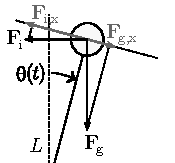
\includegraphics{fig/klatno_dinamika.pdf}
        \caption{Дијаграм динамике клатна.}
        \label{fig:\ID.2}
    \end{subfigure}
    %
    \begin{subfigure}{0.59\textwidth}
        \centering
        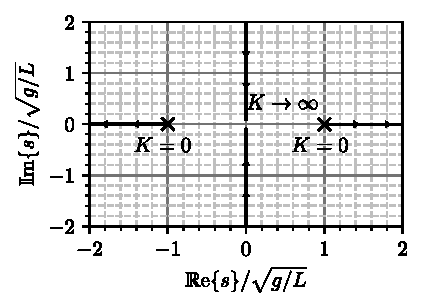
\includegraphics{fig/pmap_klatno_edit.pdf}
        \caption{Кретање полова у комплексној равни.}
        \label{fig:\ID.3}
    \end{subfigure}
\end{figure}


(б) Стабилност система се испитује на основу структуре полова функције преноса. Полови $p=s$ се потражују као корени полинома у имениоцу, односно као 
решења једначине $g - p^2L = 0$, односно $p_{1,2} = \pm \sqrt{g/L}$. Будући да се један од полова налази у левој комплексној полуравни (односно је 
$\Re{p} < 0$) систем је асимптотски нестабилан. 

(в) 
На основу датог блок дијаграма може се непосредно писати 
$Y = C(s)H(s)( X - Y )$, где су $Y = \LT{y(t)}$, $X = \LT{x(t)}$.B Одавде се може изразити 
$Y = \dfrac{C(s)H(s)}{1 + C(s)H(s)} X$, одакле се добија функција преноса 
целокупног система као $W(s) = \dfrac{C(s)H(s)}{1 + C(s)H(s)}$. Заменом болика $H(s)$ и $C(s)$ добија се 
\begin{eqnarray}
    W(s) = \dfrac{ \dfrac{Ks^2}{g - s^2L} }{ 1  + \dfrac{Ks^2}{g - s^2L}} = 
    \dfrac{ Ks^2 }{ g - s^2L + Ks^2} = \dfrac{ Ks^2 }{ g + (K-L)s^2}. 
\end{eqnarray}

(г) Полови функције преноса целокупног система налазе се као корени полинома у имениоцу $g - (L-K)p^2 = 0$, па се морају разликовати на основу 
знака $K-L$, односно је 
\begin{eqnarray}
    p_{1,2} = \begin{cases}
        \pm\sqrt{ \dfrac{g}{L-K} } &, K < L \\
        \pm\infty &, K = L \\
        \pm\jj\sqrt{\dfrac{g}{K-L}} &, K > L
    \end{cases}
\end{eqnarray}

Закључујмо да се полови ефективно „крећу“ по комплексној равни. На слици \ref{fig:\ID.3} приказан је дијаграм који илуструје ово кретање приликом 
варирања параметра $K > 0$. На основу овакве структуре корена може се закључити да је за 
$K \leq L$ систем је асимтотски нестабилан, а за $K > L$ је маргинално стабилан. 